%General
\documentclass{article}
\usepackage[utf8]{inputenc}
\usepackage{fullpage}

%Symbols
\usepackage{commath}
\usepackage{amsmath}
\usepackage{amssymb}
\usepackage{tikz}
\usetikzlibrary{arrows,automata}

%Numbering
\usepackage{chngcntr}
\usepackage{enumerate}

%Formatting
\usepackage{bussproofs}
\usepackage{hyperref}
\usepackage{amsthm}
\usepackage{mathtools}
\usepackage{alltt}
\newtheorem{theorem}{Theorem}[section]
\newtheorem{definition}[theorem]{Definition}
\newtheorem{example}[theorem]{Example}
\hypersetup{colorlinks=true}
\hypersetup{colorlinks=true}
\usepackage{graphicx}
\graphicspath{ {img/} }
\usepackage{caption}

\title{Week 7: Turing machines}
\date{\today}
\author{Rikard Hjort}

\begin{document}
\maketitle

\begin{enumerate}[(a)]
    \item 
        We assume that the input can only exist of the symbols 0, 1, 2 and 3. Specifically, we assume that the input can not contain the symbol $X$.

        We further assume that the Turing machine starts with the head at the leftmost symbol of the input.

        The transition diagram for the Turing machine is given below. In the diagram, $\square$ denotes the blank character, $a \in \set{0,1,X}$, $b \in \set{1,X,3}$ and $c \in \set{1,X}$.

        \begin{figure}[htpb]
            \centering
            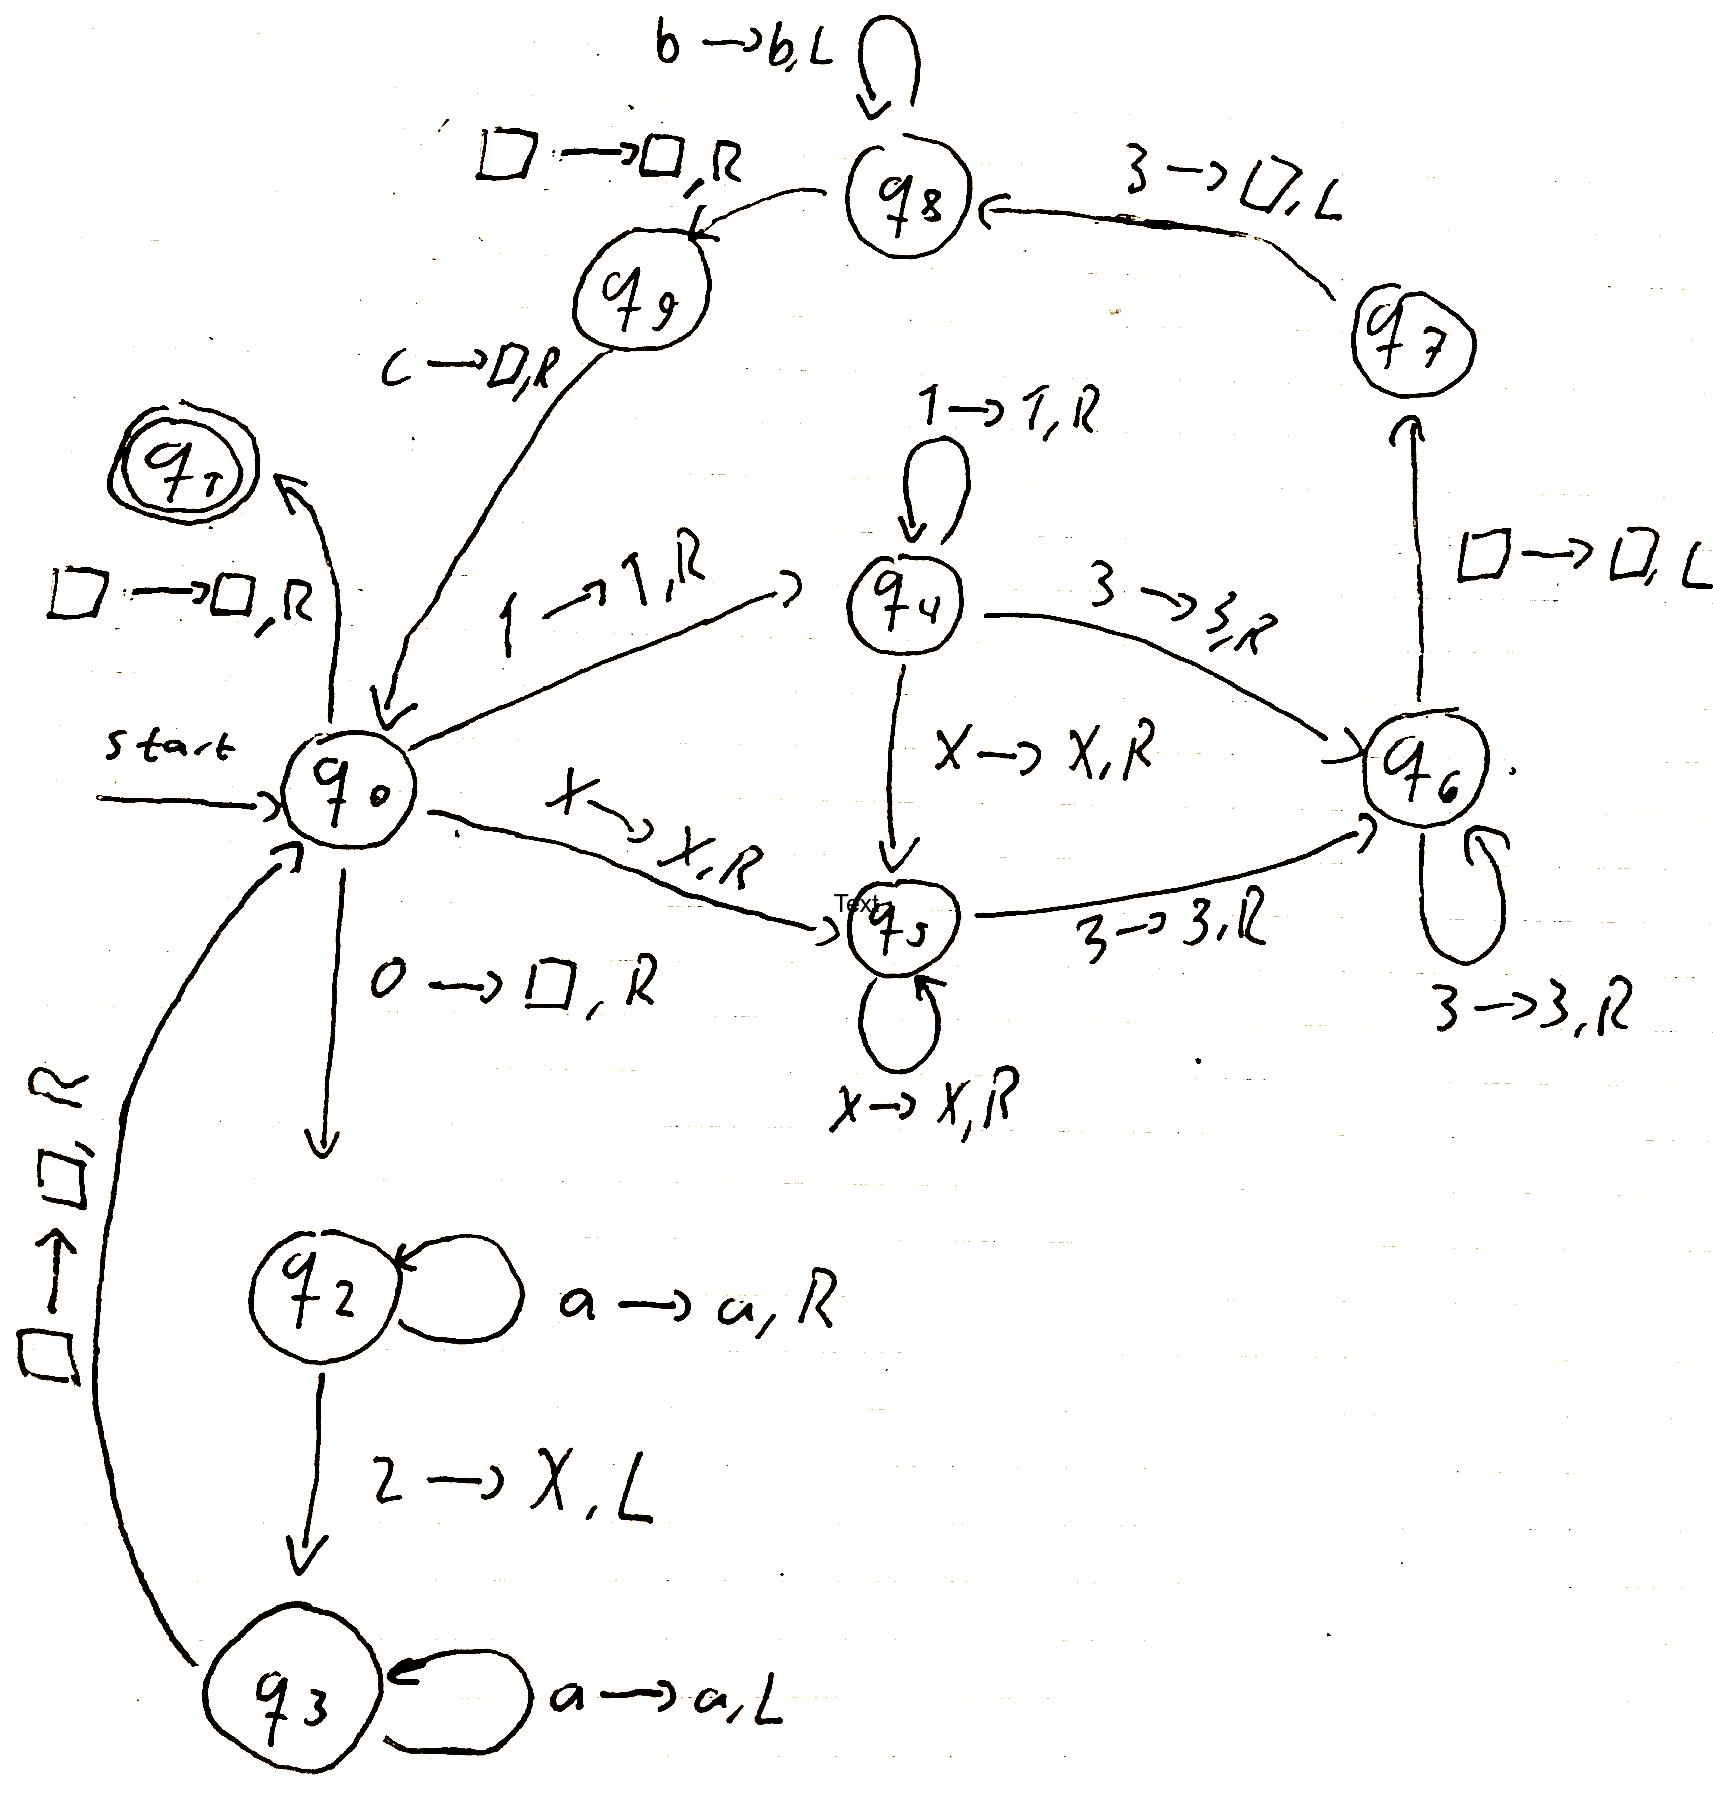
\includegraphics[width=0.75\linewidth]{turing}
            \caption{The transition diagram of the Turing machine that accepts $\mathcal{L}$.}
            \label{fig:turing}
        \end{figure}

        \newpage
    \item

        The machine operates by assuming the input is valid, and then replaces all symbols in the input with blanks in a structured process. The process of accepting a string consists of two phases. Phase 1 makes sure there are at least fewer leading 0's than there are 2's in the input. Phase 2 makes sure that the input, minus the leading 0's, had the form $(1^+2^* + 1^*2^+)3^+$, and that there were not more 2's than 0's, and also it makes sure that the number of 3's is the same as the number of 1's and 2's together. For any string that shouldn't be accepted, the machine will halt somewhere other than $q_1$.

        \textbf{A more detailed description}

        The machine starts in $q_0$. If the input is blank, the head is on a blank, and the string is valid so we accept by moving to $q_1$ and then halting. You may note that this is the only way to get to an accepting state – being at an blank symbol while in $q_0$. 
        
        If the tape is not empty, the machine will be on a non-blank symbol, and will transition out of $q_0$. The transition decides if we will enter the first phase or the second. One might think of the first phase as being represented by the big loop from $q_0$ back to itself via $q_2$ and $q_3$. The second phase is represented by the other big loop, from $q_0$ back to itself via $q_6,q_7,q_8,q_9$, and via at least one of $q_4$ and $q_5$. For any input that is in the language, each of these big loops is repeated a number of consecutive times until the phase is complete. For all other strings, the machine will at some point halt somewhere in these loops, thereby not reaching $q_1$.

        When in $q_0$, if the first symbol is a 0, the machine transitions to $q_2$. On the way, it removes the leading 0 and moves to the next symbol to the right. Now the machine loops over 0's, 1's and $X$'s, "passing" them (meaning moving over them without altering), staying in $q_2$ and moving right until a 2 is found. When  a 2 is found, it is changed to an $X$, making it "marked" as corresponding to a 0, and the machine enters $q_3$, which means that one step of this elimination is done and that the machine should start over. The machine moves the head back to the leftmost non-blank symbol on the tape and starts over.

        However, if there string now begins with a 1 or an $X$, the machine enters the second phase. If the first symbol is a 1, the machine enters $q_4$ and moves right, going over all 1's it can find and moving right. The job of $q_4$ is to "pass" all 1's. Similarly, the job of $q_5$ is to "pass" all $X$'s. Once the machine is in $q_5$, if it encounters a new 1, it halts. It is possible to skip $q_4$, meaning all 1's are gone, or to skip $q_5$ if there are no $X$'s. Finally, $q_6$ "passes" all 3's, and halts if it sees anything but 3's, making sure that the string ends in all 3's. The machine repositions itself at the end of the string by moving to $q_7$. Being in $q_7$ indicates being at the right end of a string that has the form $(1^+2^* + 1^*2^+)3^+$. From here, the machine moves to $q_8$ by eliminating the last 3 and moving left. The machine then "passes" all symbols – 1's, $X$'s and 3's – until it falls off the left end of the string. The machine repositions itself to the leftmost non-blank symbol on the tape by transitioning to $q_9$. Being in $q_9$ means a 3 has been removed, and that a corresponding 1 or $X$ may be removed. So the machine removes the first symbol.\footnote{Note that I created a new set with elements $c$ for clarity on what is being removed. In reality, we know there may only be a 1 or $X$ at this position, since we must have passed either $q_4$, $q_5$ or both, and we have not removed any 1's or $X$'s yet. So we could have used $b$ here as well.} Then the machine is once again on the first symbol from the left (or a blank if no symbols are left), and the process may be repeated.

        If the machines manages to clear the tape and return to $q_0$, then the end of the input string must have had the form $1^jX^i3^{i+j}$, since it removed 3's from one end and 1's and $X$'s from the other end. Also, since there were no 2's left during phase 2 and the machine managed to clear all 0's, there were as many 0's as 2's, so the input string is in the language.

    \newpage
    \item
        A Turing machine is a Turing decider if it is guaranteed to halt. This machine is indeed a Turing decider. Here is why.

        We begin by noting that all the loops from a state to itself in the machine can only be followed a finite number of times until the machine must switch to a new state, or halt. The motivation (rather informally) is this: Since there can only be a finite number of non-blank symbols on the tape, if the head starts on a non-blank and moves in the same direction over and over, it must at some point have no non-blank symbols more that it can pass in this fashion, so it will always reach a blank. When it reaches a blank, it must switch to a new state or halt, if it hasn't done one of these before reaching a blank. We can conclude that this particular machine can not remain in the same state forever.

        Next we prove that the machine can not follow loops of length longer than 1 indefinitely, when starting from $q_0$.

        From $q_0$, if the machine transitions to $q_1$, it will halt. 

        From $q_0$, if the machine transitions to $q_2$, it has removed one non-blank symbol. In all other transitions before coming back to $q_0$, it will either leave the symbol on the tape the way it is, or change a 2 to an $X$. None of these steps add more non-blank symbols to the tape. So upon returning to $q_0$, there is one less non-blank on the tape.

        From $q_0$, if the machine transitions to $q_4$ or $q_5$, it changes nothing, and the same when transitioning to $q_6$ and $q_7$. On transitioning to $q_8$, it removes one symbol from the end. It then changes nothing on the tape until it transitons back to $q_0$, at which point it eliminates a single symbol. So after returning to $q_0$ in this fashion, there are two less non-blanks on the tape.

        There are no other loops in the transition diagram than those of the phases, except for the edges from a state to itself that we have already shown can't be followed forever. So unless the machine halts somewhere in phase 1 or phase 2, it must return to $q_0$ with at least one less symbol left on the tape, meaning it can't keep returning to $q_0$ forever. It follows that the machine halts for all possible input, which makes it a Turing decider.
\end{enumerate}

\end{document}
